\documentclass[14pt]{extarticle}
\usepackage{graphicx} % Required for inserting images
\usepackage{multicol} % Required for multiple columns
\usepackage{multirow}
\usepackage{ragged2e} % Required for alignment
\usepackage{float}
\usepackage{extsizes}
\usepackage{tabularray}
\usepackage{color}
\usepackage{booktabs}
\usepackage[english]{babel}
\usepackage{csquotes}
\usepackage{biblatex}
\addbibresource{saranya.bib}
\renewcommand*\contentsname{TABLE OF CONTENTS}
\setcounter{secnumdepth}{0}
\tolerance=1 
\emergencystretch=\maxdimen 
\hyphenpenalty=10000
\hbadness=10000
\usepackage{geometry}
\geometry{
 a4paper,
 total={170mm,257mm},
 left=30mm,
 right=20mm,
 top=35mm,
 bottom=50mm
 }
\usepackage{setspace}
\usepackage[dvipsnames]{xcolor}

%DEFINING VARIABLES
\def\name{M Saranya}
\def\study{Comparison of Early Versus Late Amniotomy with Immediate Oxytocin Infusion In Nulliparous women with bishop’s score $\leq$6 - A Randomised Trial} 
\def\guide{Dr. P Amudha MDOG}
\def\guidedes{Professor and Head of Department}
\def\regno{???????????}
\def\date{SEPTEMBER 2026}
%DEFINING VARIABLES

\pagecolor{RoyalBlue}
\title{\study}
\author{\name}
\doublespacing

\begin{document}

\begin{center}

\textbf{\study}
\thispagestyle{empty}
\begin{figure}[hbp]
    \centering
    
\includegraphics[scale=0.75]{tnmgr_logo.png}
\end{figure}

\begin{bfseries}
\begin{spacing}{2}
REGISTRATION NO: \regno

DISSERTATION SUBMITTED TO \par THE TAMIL NADU DR. MGR MEDICAL UNIVERSITY \par IN PARTIAL FULFILMENT OF THE REQUIREMENTS FOR THE AWARD OF THE DEGREE OF \par M.S. OBSTETRICS AND GYNAECOLOGY \par Branch II \par \date
\end{spacing}
\end{bfseries}

\end{center}
\newpage
\pagecolor{white}
\thispagestyle{empty}
\begin{center}

\textbf{\study}

\begin{figure}[hbp]
    \centering
    
\includegraphics[scale=0.75]{tnmgr_logo.png}
\end{figure}

\begin{bfseries}
\begin{spacing}{2}
REGISTRATION NO: \regno

DISSERTATION SUBMITTED TO \par THE TAMIL NADU DR. MGR MEDICAL UNIVERSITY \par IN PARTIAL FULFILMENT OF THE REQUIREMENTS FOR THE AWARD OF THE DEGREE OF \par M.S. OBSTETRICS AND GYNAECOLOGY \par Branch II \par \date
\end{spacing}
\end{bfseries}
\end{center}

\newpage

\null
\setcounter{page}{1}
\pagenumbering{roman}
\centerline{\underline{{\Large\textbf{DECLARATION}}}}

\vspace{7mm}
In the following pages is presented a consolidated report of the study of ``\study'', on cases studied and followed up by me at Government Raja Mirasudhar Hospital, Thanjavur Medical College  from 2025 - 2026. This thesis is submitted to the DR. MGR Medical University, Chennai in partial fulfillment of the rules and regulations for the award of MS Degree examination in Obstetrics and Gynaecology.

\vspace{12mm}
\begin{flushright}
\textbf{\name} \\ Junior Resident, \\ Department of Obstetrics and Gynaecology, \\Government Raja Mirasudhar Hospital\\ Thanjavur Medical College, Thanjavur \\ Tamil Nadu 
\end{flushright}

\newpage

\null

\centerline{\underline{{\Large\textbf{CERTIFICATE BY THE GUIDE}}}}

\vspace{7mm}
This is to certify that this dissertation entitled {\small ``\study''} is a
bonafide \\ research work done by \name, under the guidance and supervision in
the Department of Obstetrics and Gynaecology during the period of her postgraduate study for M.S. (Obstetrics and Gynaecology) from 2023 to 2026.

\vspace{20mm}
\begin{flushright}
{\small SIGNATURE OF THE GUIDE\\[5pt]\textbf{\guide}, \\[5pt]\guidedes, \\ Department of
Obstetrics and Gynaecology \\ Government Raja Mirasudhar Hospital \\ Thanjavur Medical
College, \\ Tamil Nadu}
\end{flushright}


\newpage

FILLER FOR PLAGIARISM ANALYSIS

\newpage

\null

\centerline{\underline{{\Large\textbf{CERTIFICATE II}}}}

\vspace{7mm}
This is to certify that this dissertation entitled "\study" of the candidate
\name, REGISTRATION NUMBER: \regno for the award of MASTER OF SURGERY in the
branch of Obstetrics and Gynaecology (BRANCH II). I personally verified the
urkund.com website for the purpose of plagiarism check. I found that the
uploaded thesis file contains from introduction to conclusion pages and result
shows 2\% of plagiarism in the dissertation.

\vspace{30mm}
\begin{flushright}
\begin{bfseries}
    GUIDE and SUPERVISOR sign with seal
\end{bfseries}
\end{flushright}

\newpage

\null

\centerline{\underline{{\large\textbf{ENDORSEMENT BY THE HOD }}}}
\vspace{3mm}
\centerline{\underline{{\large\textbf{AND }}}}
\vspace{3mm}
\centerline{\underline{{\large\textbf{HEAD OF THE INSTITUTION}}}}

\vspace{7mm}
This is to certify that this dissertation entitled``\study'' is a
bonafide research workd done by \name, under the guidance and supervision of
\guide{} \guidedes, Department of Obstetrics and Gynaecology, Goverment,
Government Raja Mirasudhar Hospital Thanjavur Medical College, Tamil Nadu

\vspace{30mm}


\begin{multicols}{2}
\begin{flushleft}
    {\small SIGNATURE OF THE HOD\\[5pt]\textbf{\guide} \\[5pt]\guidedes \\ Department of OBG\\Govt. Raja Mirasudhar Hospital\\ Thanjavur Medical College, Tamil Nadu} 
\end{flushleft}

\begin{flushleft}
    {\small SIGNATURE OF THE DEAN\\[5pt]\textbf{Dr. DEAN} \\ Government Raja
    Mirasudhar Hospital, Thanjavur Medical College, \\ Tamil Nadu} 
\end{flushleft}
\end{multicols}


\newpage
\null

\centering\tableofcontents

\newpage
\justifying
\pagenumbering{arabic}
\setcounter{page}{1}

\null
\vfill
\begin{flushright}
\raggedleft\section{INTRODUCTION}
\end{flushright}
\hrulefill

\newpage
\justifying
Induction of labour is defined as the process of artificial initiation of uterine contraction, prior to spontaneous onset with intention to make progressive effacement and dilatation of cervix. Induction of labour is a commonly performed obstetric procedure. 
\newpage
\null
\vfill
\begin{flushright}
    \section{AIM OF THE STUDY}
\end{flushright}
\hrulefill
\newpage

PRIMARY OBJECTIVE:

To compare the time interval between oxytocin induction to delivery interval in women with early and late amniotomy

SECONDARY OBJECTIVE:

1. To compare the maternal and neonatal outcome in women with early and late amniotomy 

\newpage
\null
\vfill
\begin{flushright}
    \section{JUSTIFICATION FOR THE STUDY}
\end{flushright}
\hrulefill
\newpage

TBD

\newpage

\null
\vfill
\begin{flushright}
    \section{MATERIALS AND METHODS}
\end{flushright}
\hrulefill
\newpage

\textbf{\large SELECTION OF CASES:} 
\vspace{5mm}
\par This is a randomised controlled open label clinical intervention trial conducted at the Department of Obstetrics and Gynaecology, Government Raja Mirasudhar Hospital attached to Thanjavur Medical College from September 2024 to August 2025 including women admitted in the labour room who satisfy the inclusion and exclusion criteria. Patient identity will be kept confidential. Access to records for persons other than researchers and guide will be prohibited.

\vspace{5mm}

\textbf{\large INCLUSION CRITERIA}
\begin{itemize}
    \item Age $>$18 years and $\leq$35 years
    \item nulliparous women
    \item Full term >37 weeks gestation
    \item Singleton pregnancy
    \item Fetus in cephalic presentation
    \item Bishop’s Score$\geq$6
    \item Reassuring fetal heart rate.
\end{itemize}

\textbf{\large EXCLUSION CRITERIA}
\begin{itemize}
    \item multiparous women
    \item History of uterine surgery
    \item Ruptured membranes
    \item Macrosomia
    \item Gross congenital malformation,
    \item Estimated fetal weight<3rdpercentile
    \item HIV
    \item Hepatitis B or C.
\end{itemize}

\textbf{\large SAMPLE SIZE:}

140 women admitted for induction of labour who fulfill the inclusion criteria.70 among early amniotomy group,70 among late amniotomy group.

\textbf{\large STATISTICAL METHODS:}

Informed consent was obtained from the patients. A detailed history and physical examination of the patients was done. Thorough clinical examination including recording of vital parameters, systemic and obstetric examination was done. The modified biophysical profile and per vaginal examination to assess  cervical ripening is done for all patients. Women with Bishop’s score of $\geq$6,who fulfill the inclusion criteria were enrolled for the study. After inclusion, each woman was assigned randomly to either early amniotomy or late amniotomy. Group 1 consisted of women who had amniotomy soon after randomization and immediate oxytocin infusion. Group 2 consisted of women who hadd induction of labour with oxytocin infusion and amniotomy was performed 4 hours later.

Oxytocin infusion was started at a concentration of 5 mIUnits/min, the time of oxytocin commencement will be recorded. After 4 hours of oxytocin infusion in the early amniotomy group participants were reviewed and cervical  assessment performed. In the delayed aminotomy group Artificial rupture of Membrane will be done  if it is still intact. If in case membrane ruptured either during cervical ripening phase or within 4 hours of oxytocin infusion, those mothers were excluded from the study. In the event of non -reassuring CTG or uterine hyperactivity either oxytocin infusion will be reduced or stopped and delivery will be expedited depending on the individual circumstances. Subsequent management of labour and decision for operative delivery will be at the discretion of labour ward care provider and same will be recorded. Neonatal data like Birth weight, Apgar score, NICU Admission and reason for admission were also recorded. The results were entered in a spreadsheet. Descriptive analysis was done for descriptive data. A two-tailed student t test was performed on continuous data. p-value of $\leq$0.05 was considered significant.

\newpage
\null
\vfill
\begin{flushright}
    \section{REVIEW OF LITERATURE}
\end{flushright}
\hrulefill
\newpage

review of literature
wrte about natura labour progression
write about amniotomy as a procedure
werite about oxytocin
and other labour induction methods

\textbf{LABOUR}

Labour in obstetrics is the process by which the fetus is expelled out of the birth canal as a result of a series of changes involving but not limited to primarily uterus and cervix. Labour ,although takes place within a span of a few hours, involves extensive preparation begin several days to weeks prior. The processes involved in the initiation and progression of labour are not completely understood. Various theories have been proposed to explain the physiology of labour, all of which focus mainly on the following factors 

\begin{itemize}
    \item functional loss of pregnancy maintenance factors
    \item synthesis of factos that induce parturition
    \item fetal source of signal for parturition commencement
\end{itemize}

Labour has also been described in terms of three P's namely "Power", "passenger" and "passage". Successful labour depends on the coordinated changes occuring in these three factors. Labour has moreover been differentiated into fours stages based on cervical dilatation, uterine contraction and the position of the fetus and placental membranes. All these divisions serve to characterize normal labour from pathological labour.

\textbf{PHYSIOLOGY OF LABOUR}

The physiology of labour is explained in terms of changes occuring in the uterus, cervix and the placenta, changes in the endocrinology of the mother and fetus and various other local factos most important of which are prostaglandins \cite{myattExpressionLocalizationFunction2004}. In order to explain the various factors at play in the initiation and progress of labour, pregnancy is classified into four phases namely

\begin{itemize}
    \item Phase of uterine quiescence 
    \item Phase of Activation
    \item Phase of Stimulation 
    \item Phase of Involution
\end{itemize}

\textbf{Phase I - Phase of Uterine Quiscence}

The first phase of parturition - the phase of uterine quiescence is characterized by uterine unresponsiveness and smooth muscle inhibition in order to accomodate the growing fetus. This phase of labour starts even before implantation and is seen through 95\% of the pregnancy. The uterine smooth muscle undergoes extensive modification that renders it resistant to stimuli. This state of myometrial tranquility is promoted by many factors including but not limmited to 

\begin{itemize}
    \item progesterone 
    \item estrogen
    \item increase in cAMP
    \item increase in cGMP
    \item reduction in intracellular Ca2+
    \item activation of stress unfolded proterin response by uterine endoplasmic reticulum
    \item accelerated uterotonin degradation
\end{itemize}

This causes the actin in the smooth muscle to take a globular form instead of filamentous form which results in the relaxation of the muscle fibre. This is aided by the reduction in Calcium ions inside the cell. Modulation of ion channels including sodium, calciun and potassium channels result in efflux of these ions results in reduced membrane potential thus reducing contractility. Of notable mention among these channels are the sodium leak channels (NALCN) and the large conductance voltage and calcium activated potassium channel (BK\textsubscript{Ca}). Progesterone reduced uterine contractility by reducing Contraction Associated Proteins(CAP) which include oxytocin receptor, prostaglanding F receptor and connexin -43, a myometrial gap junction, and increasing anticontractile agents such as caspase 3 \cite{wuProgesteroneReceptorSignaling2017}. During labour these CAPs increase and increase uterine contractility. 

G protein couple receptor through various pathways, acting in conjuction with sex steroid hormones maintain quiesence \cite{priceAdenylylCyclaseIsoforms2000}. Higher levels of LH and HCG which share the same receptor act on these G-protein coupled receptor and play a role in uterine quescence \cite{ambrusNovelRegulationPregnant1994a}. Beta Adrenergic receptors also cause myometrial quescience in a similar fashion and this effect is utilised in tocolysis.

The decidua is the transition zone between the mother and fetus both anatomically and functionally. The decidua serves as a barrier between the mother and fetus, protecting the fetus from the immune system of the mother by altering the functioning of immune cells like NK cells, dendritic cells and macrophages \cite{anderImmuneResponsesMaternalfetal2019}.

In phase I there is softening of cervical stroma also called Hegar's sign. This occurs as early as 4-6 weeks serving as a sign of pregnancy. This happens as a result of changes in the Extra cellular matrix of the cervix \cite{nallasamyDistinctRolesCervical2017} specifically a reduction in the cross-links between the ECM proteins \cite{akinsCervicalSofteningPregnancy2011}. This is further strengthened by the fact that patients with congenital defects in these ECM proteins are prone for cervical insufficiency \cite{anumConnectiveTissueRelated2009}.  


\textbf{PHASE 2 - PHASE OF PREPARATION FOR LABOUR}     

Phase 2 is characterized by myometrial activation. This phase spans the last few weeks of parturition. The main changes in the phase 2 of parturition includes 

\begin{itemize}
    \item progesterone withdrawal
    \item myometrial preparation
    \item cervical ripening
    \item fetal maturation
\end{itemize}

Progesterone, one of the factors responsible for maintaining the uterine quescience in the first phase of parturition is withdrawn in the second phase thus reducing the uterine resistance to contractility factors. This progesterone withdrawal is brought about by selective expression of progesterone receptor isoforms, local inactivation of progesterone by natural progesterone antagonists, up regulation of progesterone metabolizing enzymes among other mechanisms \cite{ProgesteroneWithdrawalEstrogen}. The fact that administration of Mifepristone, a progesterone receptor antagonists promotes labour and abortion reiterates the importance of progesterone withdrawal in the preparation of the uterus for labour. 

Progesterone withdrawal mediates a cascade of events that result in the activation of proteins called Contraction Associated Proteins(CAPs) \cite{nadeemMolecularEvidenceFunctional2016}. The selective expression of CAPs, depending on the location of uterus, serves to differentiate the upper segment from the lower segment of the uterus \cite{wilsonProgesteroneSignalingMyometrial2020} . CAPs are expressed more in the upper segment of the uterus while CAPs are found in lower quantities in the lower uterine segment. This helps in the relative relaxation of the lower uterine segment thus aiding in expelling the fetus outside of the uterus at term. Moreover progesterone inhibits oxytocin receptor expression and therefore in phase 2 there in increase in the expression of oxytocin receptors. This increases the sensitivity of the uterus to oxytocin.

Cervical changes in the second phase of labour results in a process called cervical ripening. This is brought about mainly by change in the composition of glycosaminoglycans in the stroma of the cervix. Glycosaminoglycans absorb water and this results in the softening of the cervix which results in the ripening of the cervix \cite{akgulHyaluronanCervicalEpithelia2014}. 

The fetus plays an active part in signalling the uterus and cervix of its readiness to be expelled from the uterine cavity. The main methods by which the fetus expresses its signals is by

\begin{itemize}
    \item mechanical
    \item endocrinological
    \item lung surfactant
    \item platelet activating factor
    \item fetal membranes
\end{itemize}

The increase in fetal mass increases expression of CAPs line connexins-43 and oxytocin receptor and also by changing the composition of ions channels and cell surface receptors on the surface of myometrial cells. This signalling pathway is called Mechanotransduction. This results in breaking the myomtrial quescience thus aiding in the advancement of parturition to phase 2. Increase in mass of the uterine cavity in conditions like  polyhydramnios, multiple gestation results in preterm labour. 

Endocrinological factors that result in the progression to phase 2 of parturition involves mainly cortisol and more importantly placental CRH. Cortisol which has a negative feedback on the hypothalamic CRH has an inverse relation with placental CRH. Increase in cortisol results in a feed forward loop that stimulates placental CRH. This cascade of events continue till delivery and fall almost immediately after delivery. CRH levels are lowest in the first trimester and increase constantly over the course of pregnancy. Its effects are offset by the CRH binding protein (CRH-BP) which binds and inactivates circulating CRH. A fall in the CRH-BP level at the end of pregnancy triggers events that lead to the progression of labour. CRH levels are also influenced by oxytocin levels.




\newpage
\null
\vfill
\begin{flushright}
    \section{RESULTS}
\end{flushright}
\hrulefill
\newpage

\begin{table}[ht]
\centering
\begin{tabular}{|l|c|c|c|}
\hline
\textbf{}                                                  & \multicolumn{1}{l|}{\textbf{MEAN(yrs)}} & \multicolumn{1}{l|}{\textbf{STD DEV(yrs)}} & \multicolumn{1}{l|}{\textbf{p-value}} \\[10pt] \hline
\begin{tabular}[c]{@{}l@{}}Early\\[10pt]  Amniotomy\end{tabular} & 25.91                                   & 5.45                                       & \multirow{2}{*}{0.9606}               \\ \cline{1-3}
\begin{tabular}[c]{@{}l@{}}Late \\[10pt] Amniotomy\end{tabular}  & 25.96                                   & 4.77                                       &                                       \\ \hline
\end{tabular}
\caption{Table showing the age distribution in the study population.}
\end{table}

\begin{figure}[!hb]
\begin{center}
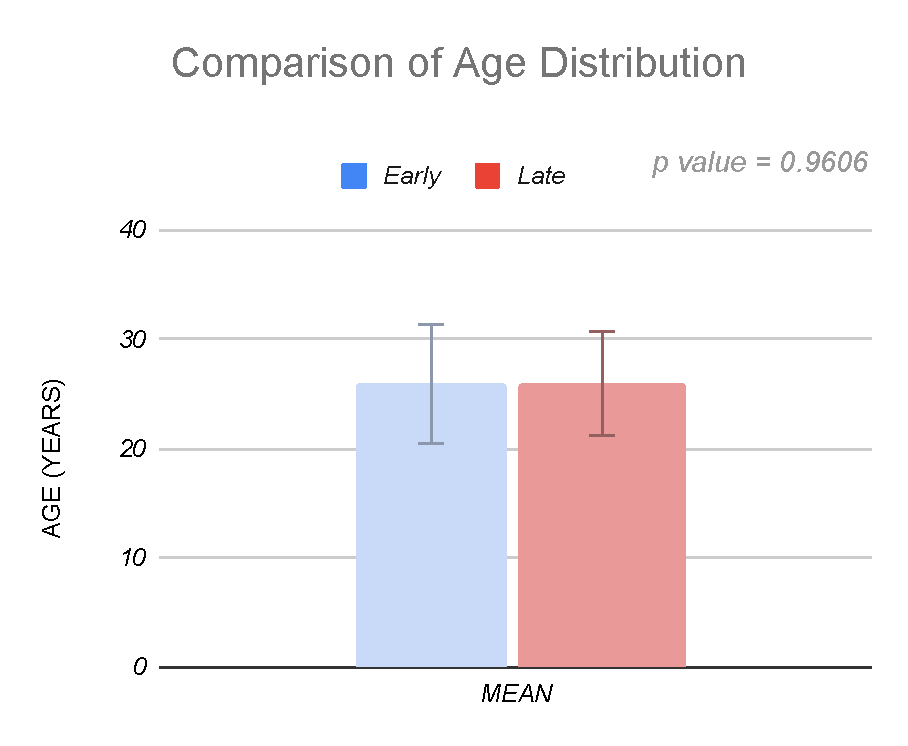
\includegraphics[width=0.95\textwidth]{figures/saranya_1}
\end{center}
\caption{Chart showing the age distribution in the study population.}
\end{figure}

\clearpage

\begin{table}[ht]
\centering
\begin{tabular}{|l|c|c|c|c|}
\hline
\multicolumn{1}{|c|}{\textbf{AGE GROUP}} & \textbf{EARLY (n=70)} & \textbf{(\%)} & \textbf{LATE (n=70)} & \textbf{(\%)} \\ \hline
\textless{}21                            & 14                    & 20            & 13                   & 18.57         \\ \hline
21-30                                    & 40                    & 57.14         & 45                   & 64.29         \\ \hline
\textgreater{}30                         & 16                    & 22.86         & 12                   & 17.14         \\ \hline
\end{tabular}
\caption{Table showing the distribution of women in different age groups in the study population}
\end{table}

\begin{figure}[!hb]
\begin{center}
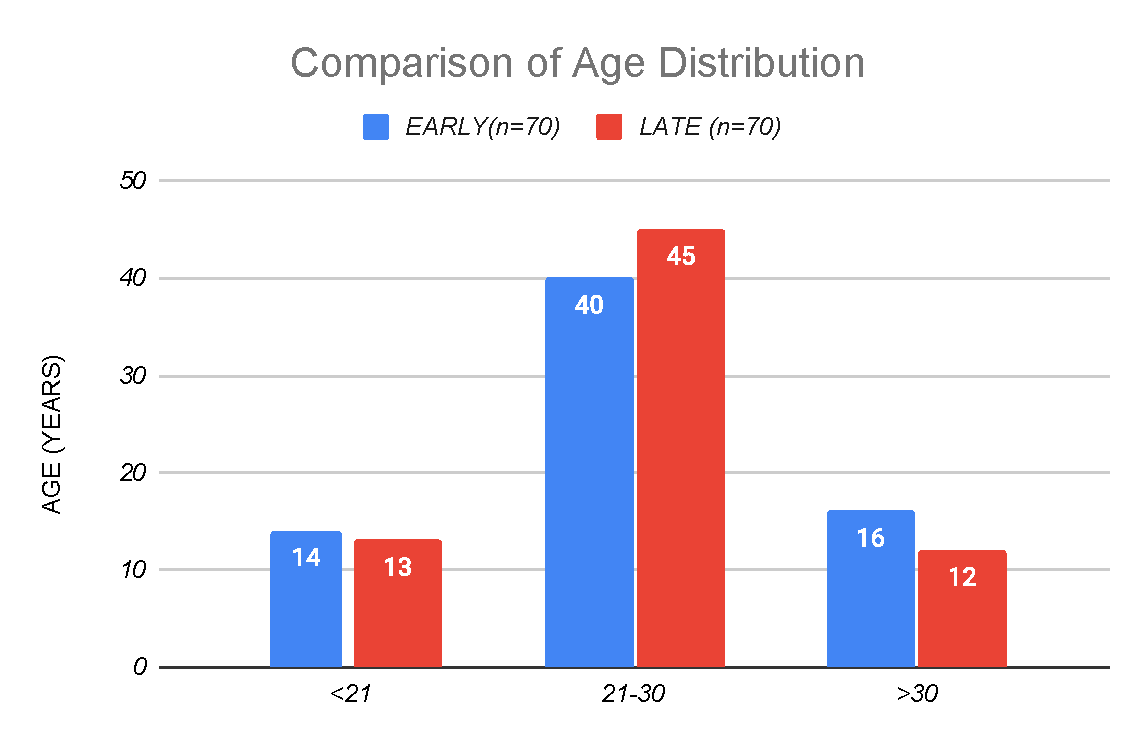
\includegraphics[width=0.95\textwidth]{figures/saranya_2}
\end{center}
\caption{Chart showing the distribution of women in different age groups in the study population}
\end{figure}
\clearpage

\begin{table}[ht]
\centering
\begin{tabular}{|l|c|c|c|}
\hline
\textbf{}                                                  & \multicolumn{1}{l|}{\textbf{MEAN}} & \multicolumn{1}{l|}{\textbf{STD DEV}} & \multicolumn{1}{l|}{\textbf{p-value}} \\ \hline
\begin{tabular}[c]{@{}l@{}}Early\\  Amniotomy\end{tabular} & 24.10                             & 3.09                                  & \multirow{2}{*}{0.3531}               \\ \cline{1-3}
\begin{tabular}[c]{@{}l@{}}Late \\ Amniotomy\end{tabular}  & 24.60                             & 3.24                                  &                                       \\ \hline
\end{tabular}
\caption{Table showing the BMI distribution in the study population.}
\end{table}

\begin{figure}[!hb]
\begin{center}
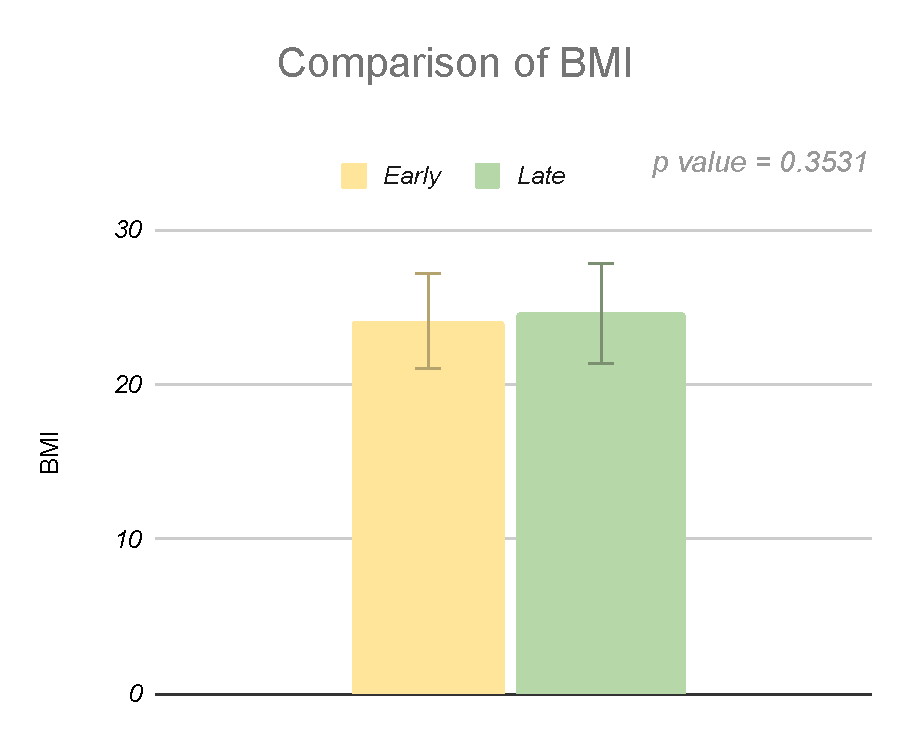
\includegraphics[width=0.95\textwidth]{figures/saranya_3}
\end{center}
\caption{Chart showing the BMI distribution in the study population.}
\end{figure}
\clearpage

\begin{table}[ht]
\centering
\begin{tabular}{|l|c|c|c|}
\hline
\textbf{}                                                  & \multicolumn{1}{l|}{\textbf{MEAN(wks)}} & \multicolumn{1}{l|}{\textbf{STD DEV(wks)}} & \multicolumn{1}{l|}{\textbf{p-value}} \\ \hline
\begin{tabular}[c]{@{}l@{}}Early\\  Amniotomy\end{tabular} & 38.61                                   & 1.17                                       & \multirow{2}{*}{0.3319}               \\ \cline{1-3}
\begin{tabular}[c]{@{}l@{}}Late \\ Amniotomy\end{tabular}  & 38.43                                   & 1.08                                       &                                       \\ \hline
\end{tabular}
\caption{Table showing the distribution of gestational age in the study population.}
\end{table}

\begin{figure}[!hb]
\begin{center}
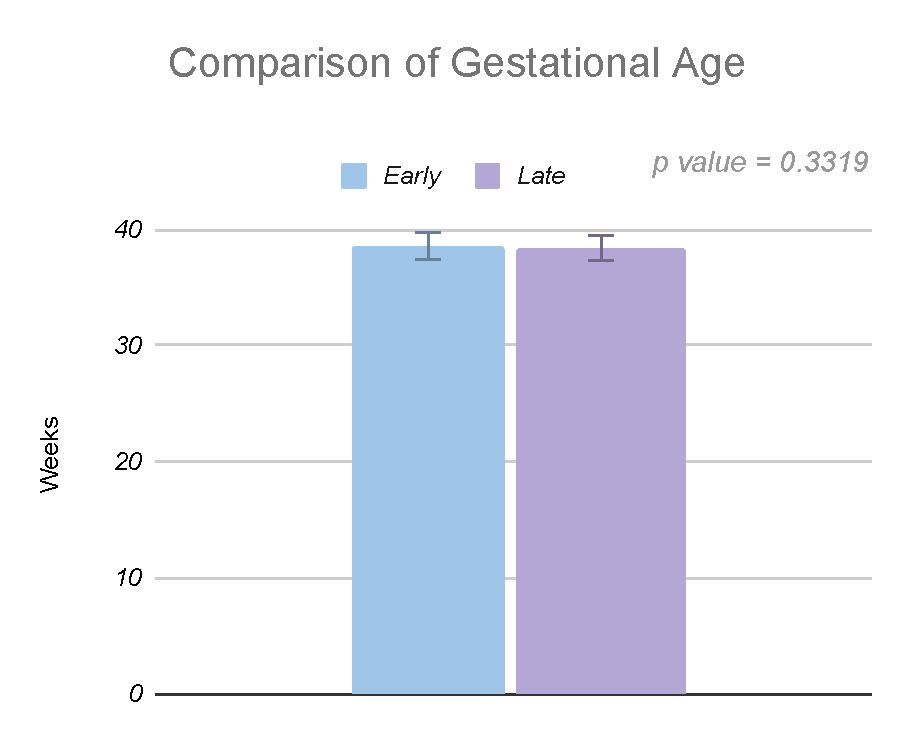
\includegraphics[width=0.95\textwidth]{figures/saranya_4}
\end{center}
\caption{Chart showing the distribution of gestational age in the study population.}
\end{figure}
\clearpage

\begin{table}[ht]
\centering
\begin{tabular}{|l|c|c|c|c|}
\hline
\textbf{\begin{tabular}[c]{@{}l@{}}INDICATION \\ FOR IOL\end{tabular}} & \textbf{EARLY (n=70)} & \textbf{(\%)} & \textbf{LATE (n=70)} & \textbf{(\%)} \\ \hline
GDM                                                                    & 22                    & 31.43         & 25                   & 35.71         \\ \hline
Post dates                                                             & 22                    & 31.43         & 15                   & 21.43         \\ \hline
Hypertension                                                           & 3                     & 4.29          & 2                    & 2.86          \\ \hline
Preeclampsia                                                           & 7                     & 10            & 6                    & 8.57          \\ \hline
Oligohydramnios                                                        & 16                    & 22.86         & 22                   & 31.43         \\ \hline
\end{tabular}
\caption{Table showing the various indication for induction of labour in the study population.}
\end{table}

\begin{figure}[!hb]
\begin{center}
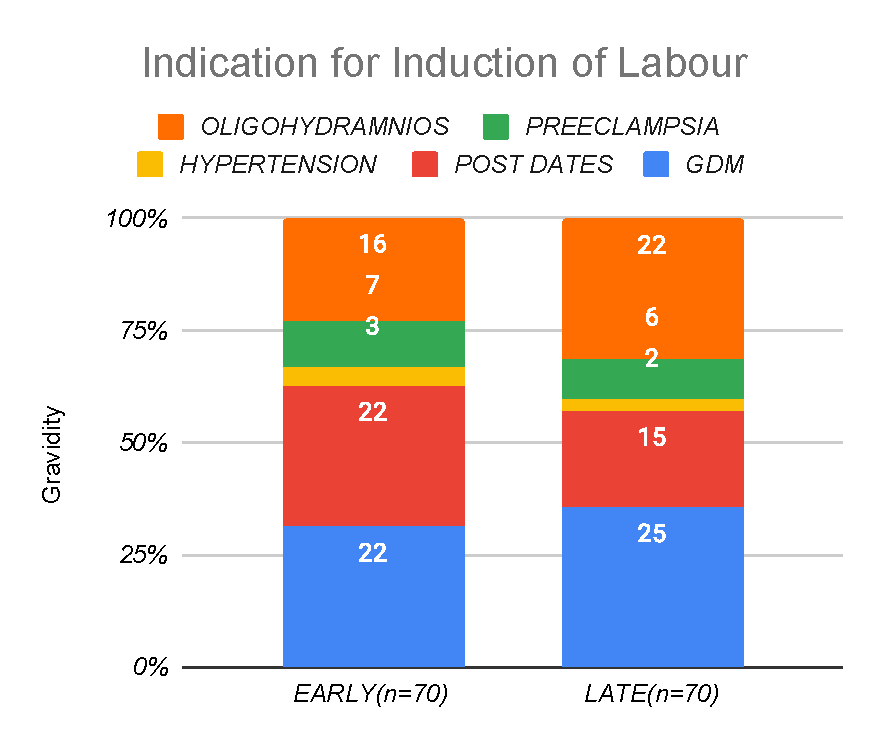
\includegraphics[width=0.75\textwidth]{figures/saranya_6}
\end{center}
\caption{Chart showing the various indication for induction of labour in the study population.}
\end{figure}
\clearpage

\begin{table}[ht]
\centering
\begin{tabular}{|l|c|c|c|}
\hline
\textbf{}                                                  & \multicolumn{1}{l|}{\textbf{MEAN}} & \multicolumn{1}{l|}{\textbf{STD DEV}} & \multicolumn{1}{l|}{\textbf{p-value}} \\ \hline
\begin{tabular}[c]{@{}l@{}}Early\\  Amniotomy\end{tabular} & 6.37                               & 0.49                                  & \multirow{2}{*}{0.6067}               \\ \cline{1-3}
\begin{tabular}[c]{@{}l@{}}Late \\ Amniotomy\end{tabular}  & 6.41                               & 0.50                                  &                                       \\ \hline
\end{tabular}
\caption{Table showing the distribution of bishop's score in the study population.}
\end{table}

\begin{figure}[!hb]
\begin{center}
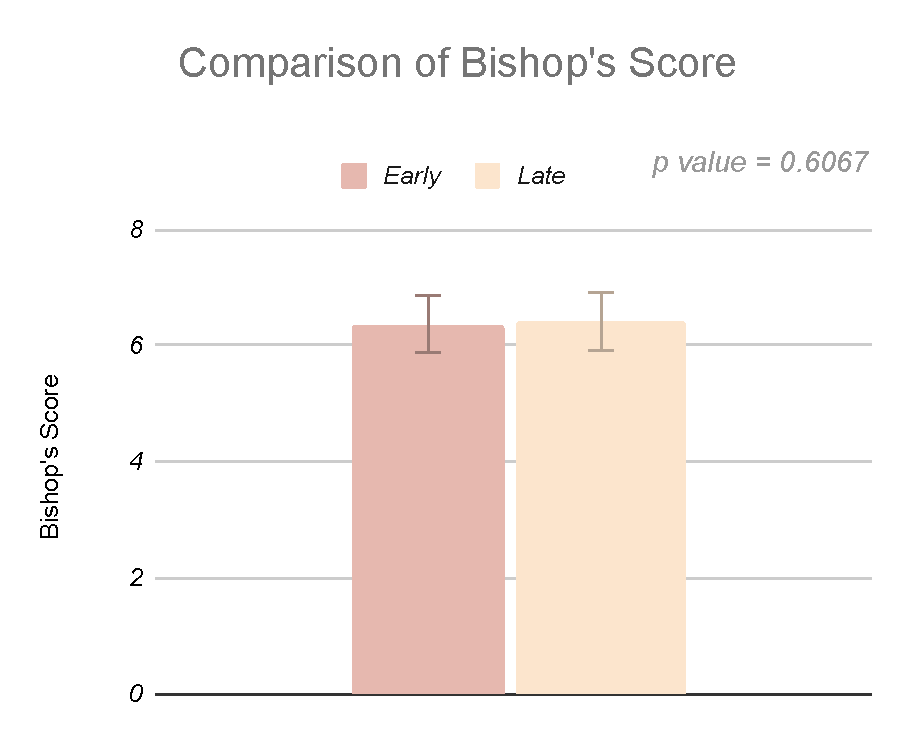
\includegraphics[width=0.95\textwidth]{figures/saranya_7}
\end{center}
\caption{Chart showing the distribution of bishop's score in the study population.}
\end{figure}
\clearpage

\begin{table}[ht]
\centering
\begin{tabular}{|l|c|c|c|}
\hline
\textbf{}                                                  & \multicolumn{1}{l|}{\textbf{\begin{tabular}[c]{@{}l@{}}MEAN\\ (hrs:min)\end{tabular}}} & \multicolumn{1}{l|}{\textbf{\begin{tabular}[c]{@{}l@{}}STD DEV\\ (hrs:min)\end{tabular}}} & \multicolumn{1}{l|}{\textbf{p-value}} \\ \hline
\begin{tabular}[c]{@{}l@{}}Early\\  Amniotomy\end{tabular} & 3:49                                                                                   & 1:30                                                                                      & \multirow{2}{*}{\textless{}0.0001}    \\ \cline{1-3}
\begin{tabular}[c]{@{}l@{}}Late \\ Amniotomy\end{tabular}  & 7:58                                                                                   & 2:57                                                                                      &                                       \\ \hline
\end{tabular}
\caption{Table showing the time taken to reach active phase in the study population.}
\end{table}

\begin{figure}[!hb]
\begin{center}
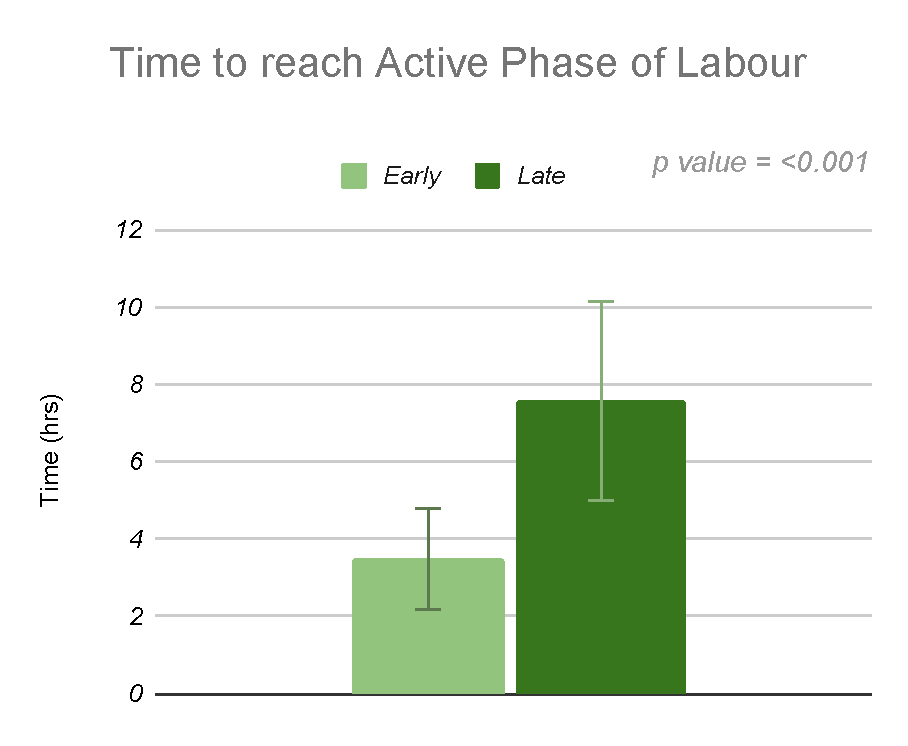
\includegraphics[width=0.85\textwidth]{figures/saranya_8}
\end{center}
\caption{Chart showing the time taken to reach active phase in the study population.}
\end{figure}

\clearpage

\begin{table}[!ht]
\centering
\begin{tabular}{|l|c|c|c|}
\hline
\textbf{} & \textbf{\begin{tabular}[c]{@{}c@{}}OXYOCIN INDUCTION \\ TO DELIVERY(hrs:min)\end{tabular}} & \textbf{\begin{tabular}[c]{@{}c@{}}STD DEV\\ (hrs:min)\end{tabular}} & \textbf{p-value}      \\ \hline
Early     & 2:16                                                                                       & 1:28                                                                 & 0.2794          \\ \hline
Late      & 1:59                                                                                       & 1:20                                                                 & \multicolumn{1}{l|}{} \\ \hline
\end{tabular}
\caption{Table showing the time interval between oxytocin induction and delivery in the study population.}
\end{table}

\begin{figure}[!hb]
\begin{center}
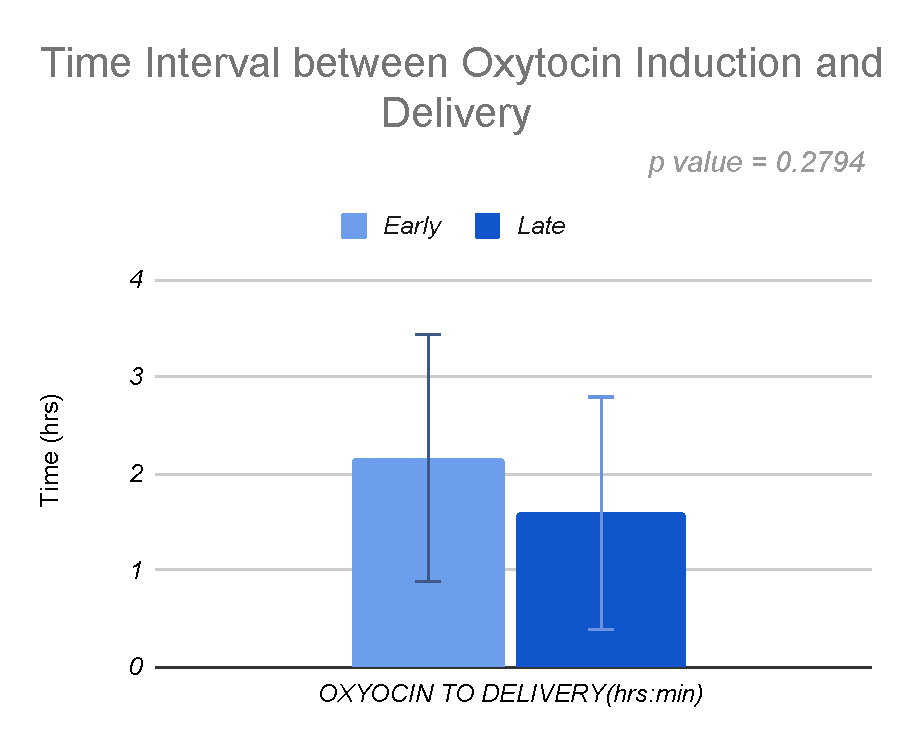
\includegraphics[width=0.95\textwidth]{figures/saranya_10}
\end{center}
\caption{Chart showing the time interval between oxytocin induction and delivery in the study population.}
\end{figure}
\clearpage

\begin{table}[!ht]
\centering
\begin{tabular}{|l|c|c|c|}
\hline
\textbf{}                                                  & \multicolumn{1}{l|}{\textbf{\begin{tabular}[c]{@{}l@{}}MEAN\\ (hrs:min)\end{tabular}}} & \multicolumn{1}{l|}{\textbf{\begin{tabular}[c]{@{}l@{}}STD DEV\\ (hrs:min)\end{tabular}}} & \multicolumn{1}{l|}{\textbf{p-value}} \\ \hline
\begin{tabular}[c]{@{}l@{}}Early\\  Amniotomy\end{tabular} & 6:06                                                                                   & 2:25                                                                                      & \multirow{2}{*}{\textless{}0.0001}    \\ \cline{1-3}
\begin{tabular}[c]{@{}l@{}}Late \\ Amniotomy\end{tabular}  & 7:58                                                                                   & 2:57                                                                                      &                                       \\ \hline
\end{tabular}
\caption{Table showing the time taken from induction to delivery in the study population.}
\end{table}

\begin{figure}[!hb]
\begin{center}
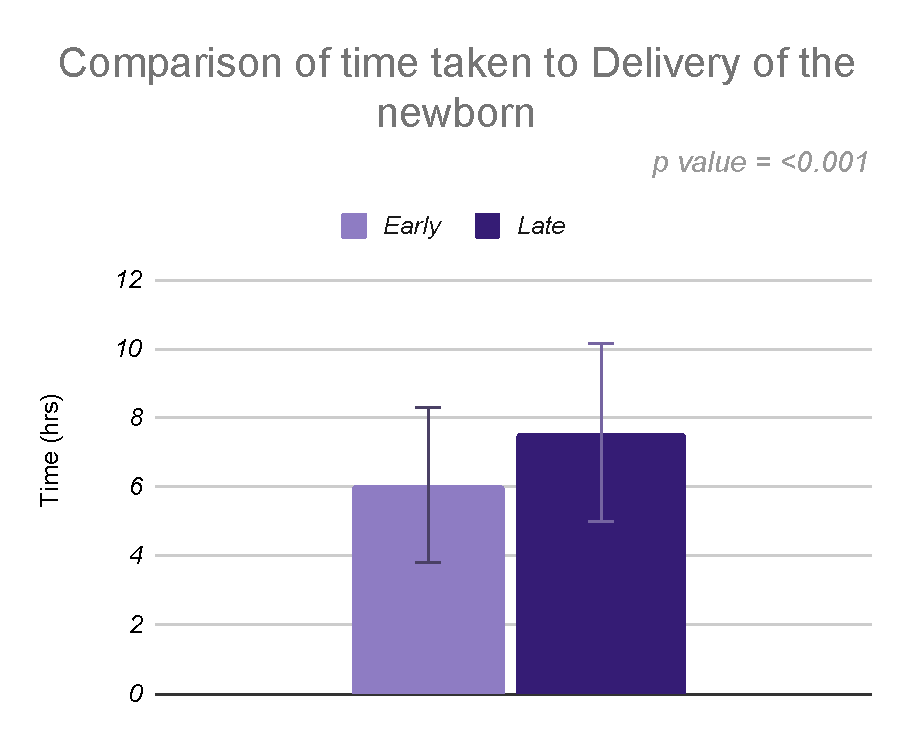
\includegraphics[width=0.85\textwidth]{figures/saranya_11}
\end{center}
\caption{Chart showing the time taken from induction to delivery in the study population.}
\end{figure}
\clearpage

\begin{table}[ht]
\centering
\begin{tabular}{|l|c|c|c|c|}
\hline
\multicolumn{1}{|c|}{\textbf{\begin{tabular}[c]{@{}c@{}}MODE OF\\  DELIVERY\end{tabular}}} & \textbf{EARLY (n=70)} & \textbf{(\%)} & \textbf{LATE (n=70)} & \textbf{(\%)} \\ \hline
Vaginal                                                                                    & 44                    & 62.86         & 31                   & 44.29         \\ \hline
Caesarean                                                                                  & 24                    & 34.29         & 38                   & 54.29         \\ \hline
\begin{tabular}[c]{@{}l@{}}Instrumental \\ Delivery\end{tabular}                           & 2                     & 2.86          & 1                    & 1.43          \\ \hline
\end{tabular}
\caption{Table showing the distribution of women in different age groups in the study population.}
\end{table}

\begin{figure}[!hb]
\begin{center}
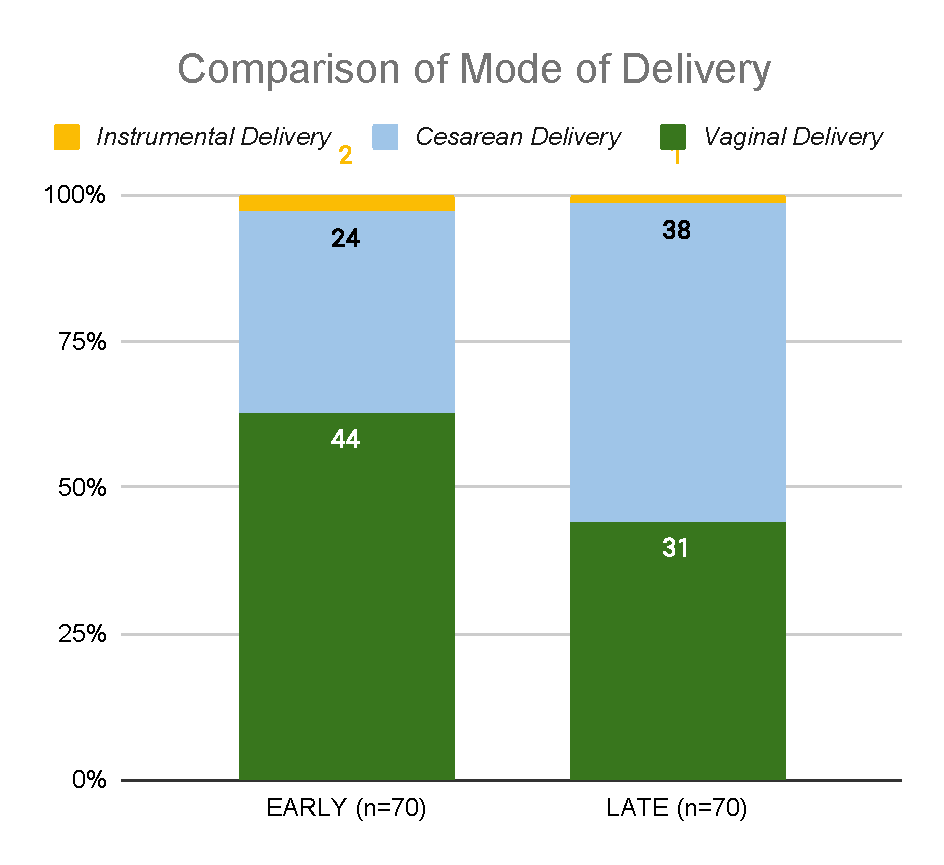
\includegraphics[width=0.75\textwidth]{figures/saranya_14}
\end{center}
\caption{Chart showing the distribution of women in different age groups in the study population.}
\end{figure}
\clearpage

\begin{table}[ht]
\centering
\begin{tabular}{|l|c|c|c|c|}
\hline
\textbf{\begin{tabular}[c]{@{}l@{}}CESAREAN \\ INDICATION\end{tabular}} & \textbf{EARLY (n=24)} & \textbf{(\%)} & \textbf{LATE (n=38)} & \textbf{(\%)} \\ \hline
Failed induction                                                            & 6                     & 25            & 15                   & 39.47         \\[10pt] \hline
Fetal distress                                                               & 14                    & 58.33         & 13                   & 34.21         \\[10pt] \hline
Arrest of labour                                                             & 4                     & 16.67         & 10                   & 26.32         \\[10pt] \hline
\end{tabular}
\caption{Table showing the various indications for caesarean section the study population.}
\end{table}

\begin{figure}[!hb]
\begin{center}
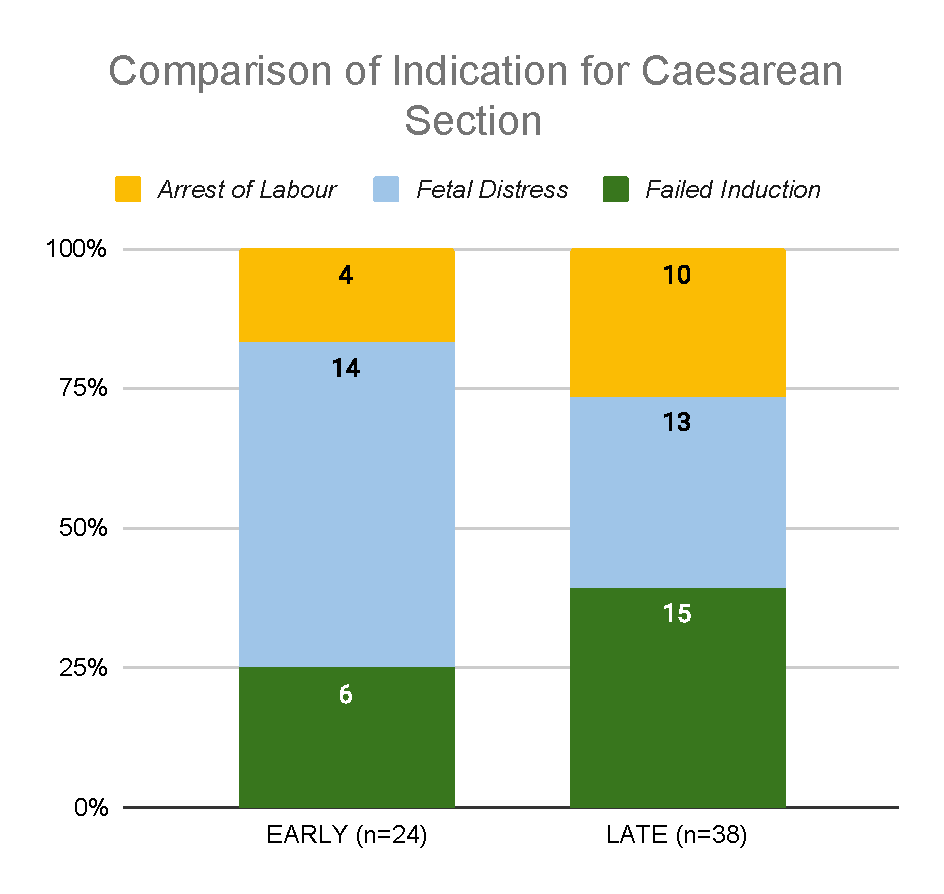
\includegraphics[width=0.75\textwidth]{figures/saranya_15}
\end{center}
\caption{Chart showing the various indications for caesarean section the study population.}
\end{figure}
\clearpage

\begin{table}[ht]
\centering
\begin{tabular}{|l|c|c|c|c|}
\hline
\textbf{\begin{tabular}[c]{@{}l@{}}CTG\\ ABNORMALITY\end{tabular}} & \textbf{\begin{tabular}[c]{@{}c@{}}EARLY \\ (n=70)\end{tabular}} & \textbf{\%} & \textbf{\begin{tabular}[c]{@{}c@{}}LATE\\  (n=70)\end{tabular}} & \textbf{\%} \\ \hline
YES                                                                & 6                                                                & 8.57        & 15                                                              & 21.43       \\[10pt] \hline
NO                                                                 & 64                                                               & 91.43       & 55                                                              & 78.57       \\[10pt] \hline
\end{tabular}
\caption{Table showing the incidence of Cardiotocographic abnormality in the study population.}
\end{table}

\begin{figure}[!hb]
\begin{center}
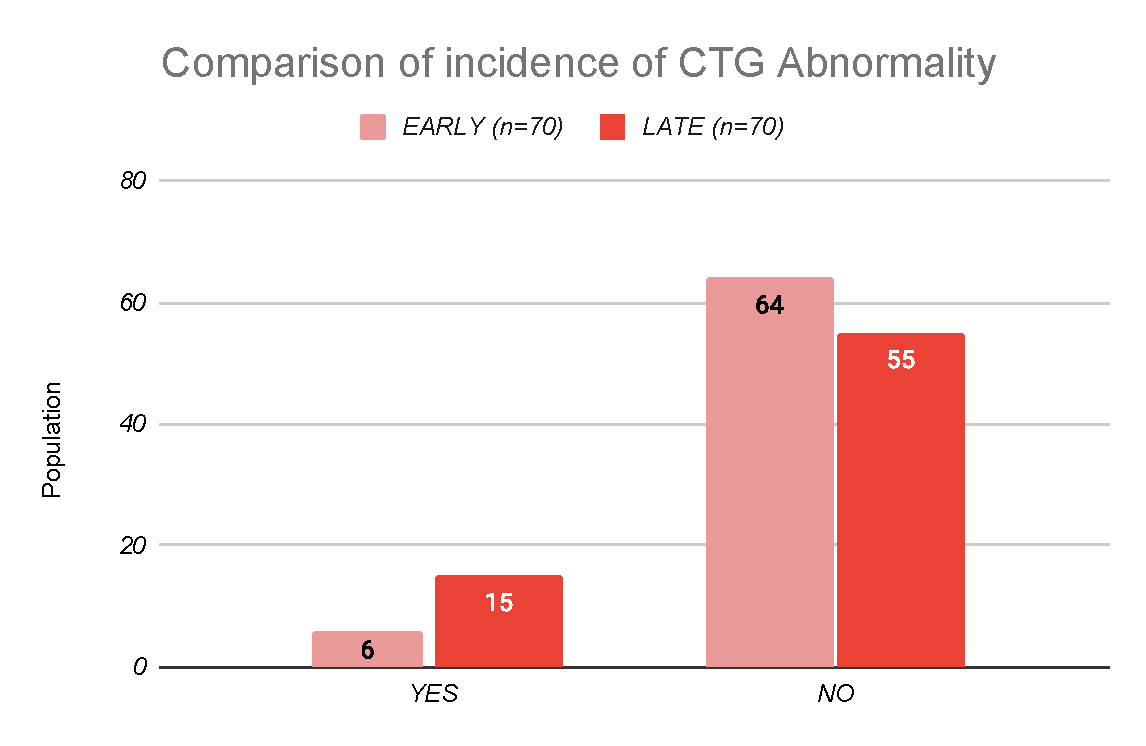
\includegraphics[width=0.95\textwidth]{figures/saranya_16}
\end{center}
\caption{Chart showing the incidence of Cardiotocographic abnormality in the study population.}
\end{figure}
\clearpage

\begin{table}[ht]
\centering
\begin{tabular}{|l|c|c|c|c|}
\hline
\textbf{\begin{tabular}[c]{@{}l@{}}UTERINE\\  HYPERSTIMULATION\end{tabular}} & \textbf{\begin{tabular}[c]{@{}c@{}}EARLY \\ (n=70)\end{tabular}} & \textbf{\%} & \textbf{\begin{tabular}[c]{@{}c@{}}LATE\\  (n=70)\end{tabular}} & \textbf{\%} \\ \hline
YES                                                                          & 1                                                                & 1.43        & 0                                                               & 0           \\[10pt] \hline
NO                                                                           & 69                                                               & 98.57       & 70                                                              & 100         \\[10pt] \hline
\end{tabular}
\caption{Table showing the incidence of post uterine hyperstimulation in the study population.}
\end{table}

\begin{figure}[!hb]
\begin{center}
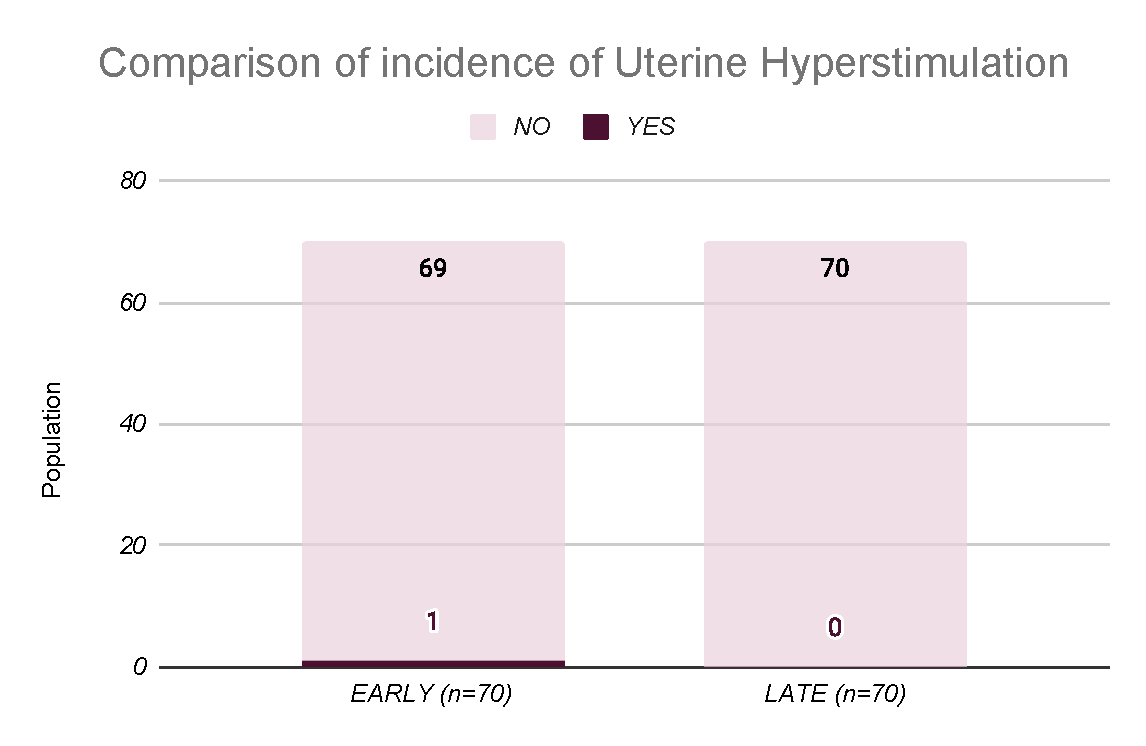
\includegraphics[width=0.95\textwidth]{figures/saranya_17}
\end{center}
\caption{Chart showing the incidence of post uterine hyperstimulation in the study population.}
\end{figure}
\clearpage

\begin{table}[ht]
\centering
\begin{tabular}{|l|c|c|c|c|}
\hline
\textbf{\begin{tabular}[c]{@{}l@{}}Post Partum\\ Hemorrhage\end{tabular}} & \textbf{\begin{tabular}[c]{@{}c@{}}EARLY \\ (n=70)\end{tabular}} & \textbf{\%} & \textbf{\begin{tabular}[c]{@{}c@{}}LATE\\  (n=70)\end{tabular}} & \textbf{\%} \\ \hline
YES                                                                       & 5                                                                & 7.14        & 9                                                               & 12.86       \\[10pt] \hline
NO                                                                        & 65                                                               & 92.86       & 61                                                              & 87.14       \\[10pt] \hline
\end{tabular}
\caption{Table showing the incidence of post partum hemorrhage in the study population.}
\end{table}

\begin{figure}[!hb]
\begin{center}
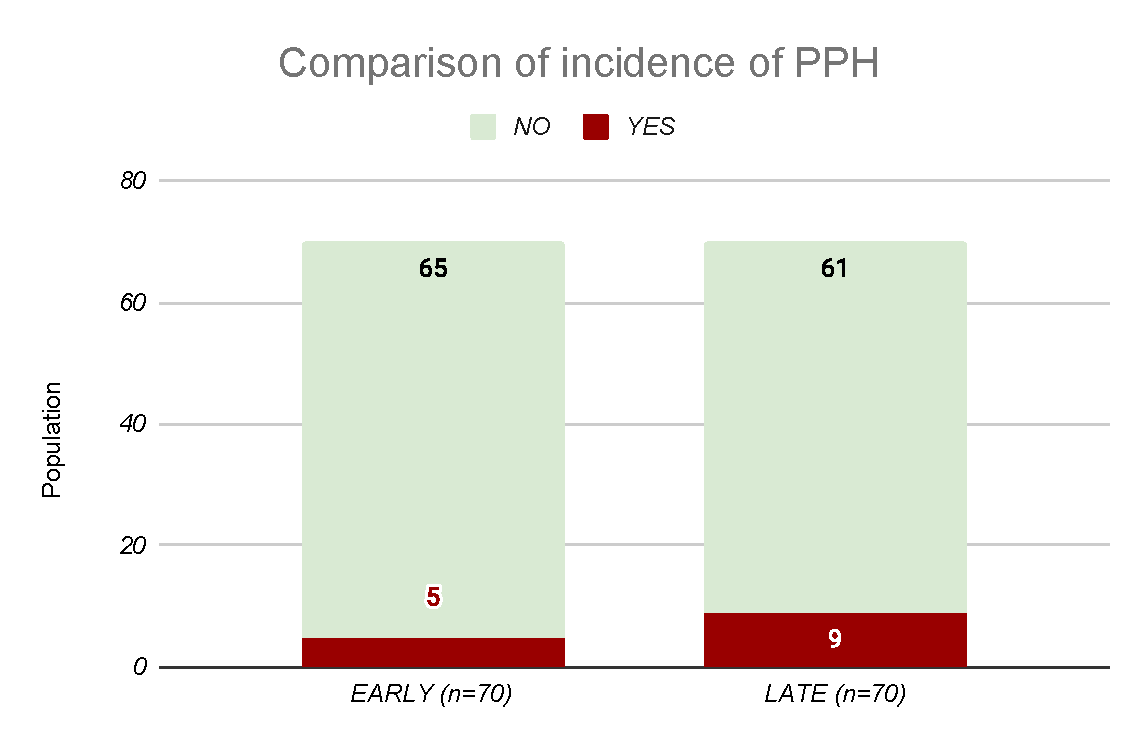
\includegraphics[width=0.95\textwidth]{figures/saranya_18}
\end{center}
\caption{Chart showing the incidence of post partum hemorrhage in the study population.}
\end{figure}
\clearpage

\begin{table}[ht]
\centering
\begin{tabular}{|l|c|c|c|}
\hline
\textbf{}                                                  & \multicolumn{1}{l|}{\textbf{MEAN(mL)}} & \multicolumn{1}{l|}{\textbf{STD DEV(mL)}} & \multicolumn{1}{l|}{\textbf{p-value}} \\ \hline
\begin{tabular}[c]{@{}l@{}}Early\\  Amniotomy\end{tabular} & 464.64                                 & 210.44                                    & \multirow{2}{*}{0.0352}               \\ \cline{1-3}
\begin{tabular}[c]{@{}l@{}}Late \\ Amniotomy\end{tabular}  & 543.21                                 & 226.38                                    &                                       \\ \hline
\end{tabular}
\caption{Table showing the the distribution of blood loss during delivery in the study population.}
\end{table}

\begin{figure}[!hb]
\begin{center}
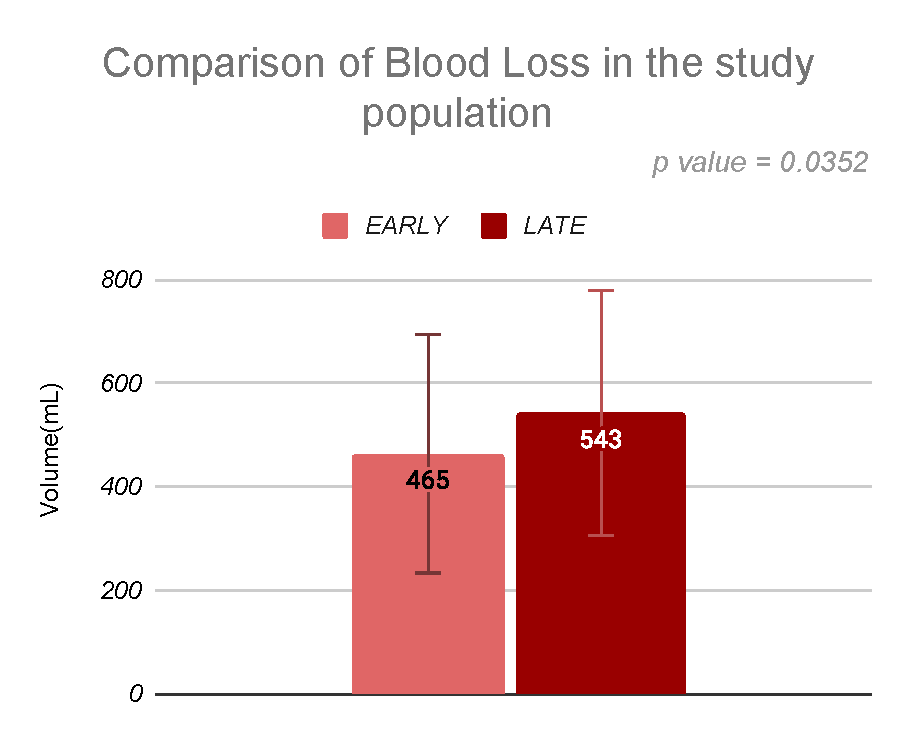
\includegraphics[width=0.95\textwidth]{figures/saranya_19}
\end{center}
\caption{Chart showing the the distribution of blood loss during delivery in the study population.}
\end{figure}
\clearpage

\begin{table}[ht]
\centering
\begin{tabular}{|l|c|c|c|}
\hline
\textbf{}                                                  & \multicolumn{1}{l|}{\textbf{MEAN(mL)}} & \multicolumn{1}{l|}{\textbf{STD DEV(mL)}} & \multicolumn{1}{l|}{\textbf{p-value}} \\ \hline
\begin{tabular}[c]{@{}l@{}}Early\\  Amniotomy\end{tabular} & 666.67                                 & 230.74                                    & \multirow{2}{*}{0.8114}               \\ \cline{1-3}
\begin{tabular}[c]{@{}l@{}}Late \\ Amniotomy\end{tabular}  & 651.97                                 & 237.91                                    &                                       \\ \hline
\end{tabular}
\caption{Table showing the the distribution of blood loss during delivery in women undergoing caesarean section in the study population.}
\end{table}

\begin{figure}[!hb]
\begin{center}
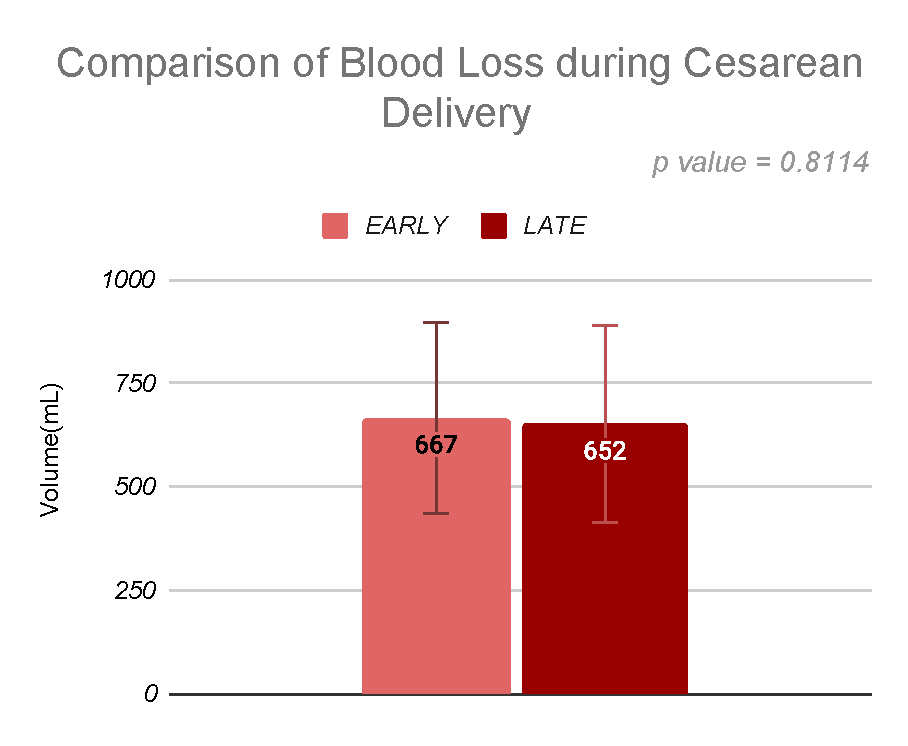
\includegraphics[width=0.95\textwidth]{figures/saranya_20}
\end{center}
\caption{Chart showing the the distribution of blood loss during delivery in women undergoing caesarean section in the study population.}
\end{figure}
\clearpage

\begin{table}[ht]
\centering
\begin{tabular}{|l|c|c|c|}
\hline
\textbf{}                                                  & \multicolumn{1}{l|}{\textbf{MEAN(mL)}} & \multicolumn{1}{l|}{\textbf{STD DEV(mL)}} & \multicolumn{1}{l|}{\textbf{p-value}} \\ \hline
\begin{tabular}[c]{@{}l@{}}Early\\  Amniotomy\end{tabular} & 359.24                                 & 86.98                                     & \multirow{2}{*}{0.0228}               \\ \cline{1-3}
\begin{tabular}[c]{@{}l@{}}Late \\ Amniotomy\end{tabular}  & 414.06                                 & 121.64                                    &                                       \\ \hline
\end{tabular}
\caption{Table showing the the distribution of blood loss during delivery in women undergoing normal vaginal delivery in the study population.}
\end{table}

\begin{figure}[!hb]
\begin{center}
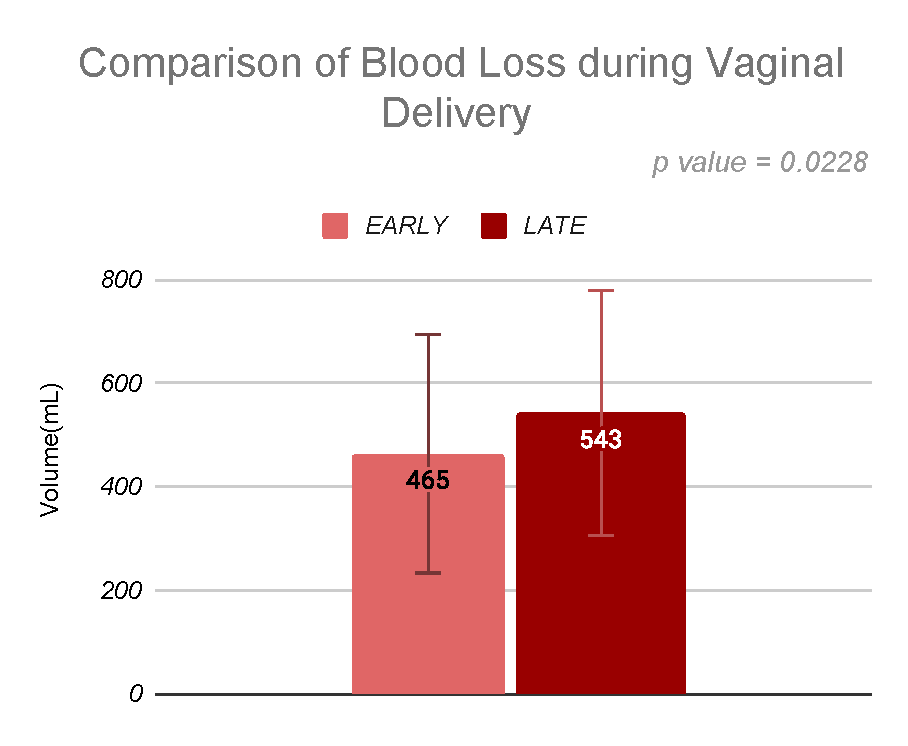
\includegraphics[width=0.95\textwidth]{figures/saranya_21}
\end{center}
\caption{Chart showing the the distribution of blood loss during delivery in women undergoing normal vaginal delivery in the study population.}
\end{figure}
\clearpage

\begin{table}[ht]
\centering
\begin{tabular}{|l|c|c|c|c|}
\hline
\textbf{\begin{tabular}[c]{@{}l@{}}MATERNAL \\ FEVER\end{tabular}} & \textbf{\begin{tabular}[c]{@{}c@{}}EARLY \\ (n=70)\end{tabular}} & \textbf{\%} & \textbf{\begin{tabular}[c]{@{}c@{}}LATE\\  (n=70)\end{tabular}} & \textbf{\%} \\ \hline
YES                                                                & 1                                                                & 1.43        & 2                                                               & 2.86        \\ \hline
NO                                                                 & 69                                                               & 98.57       & 68                                                              & 97.14       \\ \hline
\end{tabular}
\caption{Table showing the incidence of Maternal fever in the study population.}
\end{table}

\begin{figure}[!hb]
\begin{center}
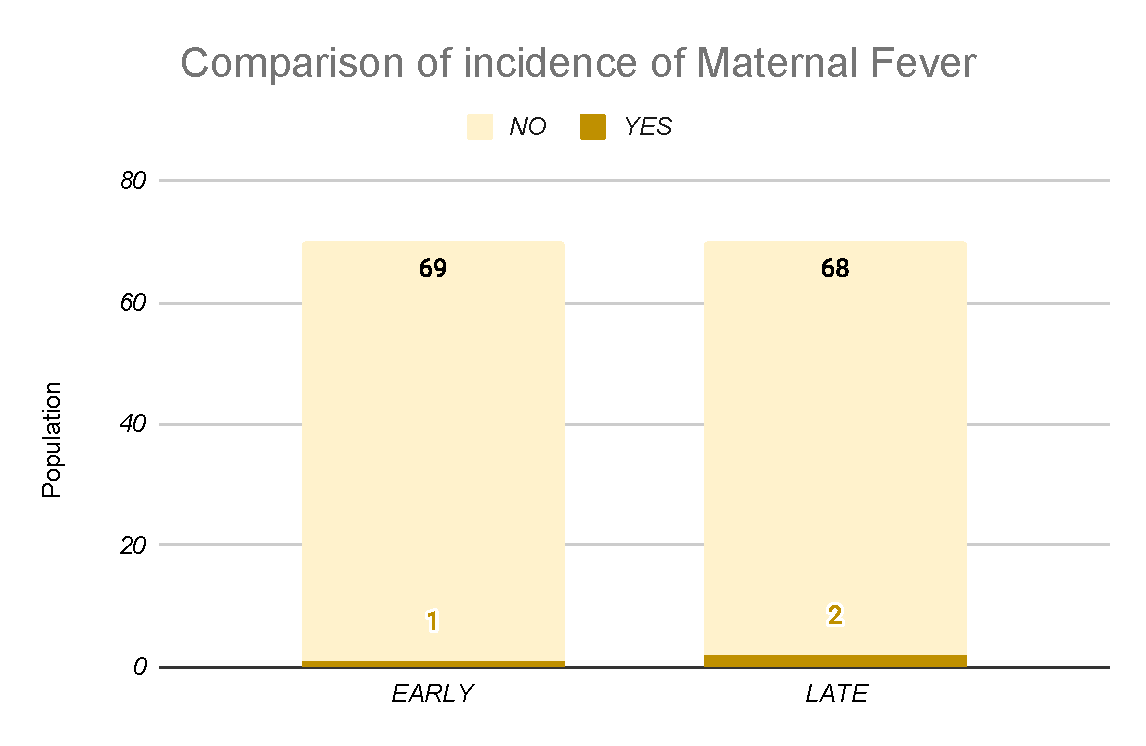
\includegraphics[width=0.95\textwidth]{figures/saranya_22}
\end{center}
\caption{Chart showing the incidence of Maternal fever in the study population.}
\end{figure}
\clearpage

\begin{table}[ht]
\centering
\begin{tabular}{|l|c|c|c|c|}
\hline
\textbf{\begin{tabular}[c]{@{}l@{}}NICU \\ ADMISSION\end{tabular}} & \textbf{\begin{tabular}[c]{@{}c@{}}EARLY \\ (n=70)\end{tabular}} & \textbf{\%} & \textbf{\begin{tabular}[c]{@{}c@{}}LATE\\  (n=70)\end{tabular}} & \textbf{\%} \\ \hline
YES                                                                & 13                                                               & 18.57       & 22                                                              & 31.43       \\ \hline
NO                                                                 & 57                                                               & 81.43       & 48                                                              & 68.57       \\ \hline
\end{tabular}
\caption{Table showing the incidence of NICU admission in the study population.}
\end{table}

\begin{figure}[!hb]
\begin{center}
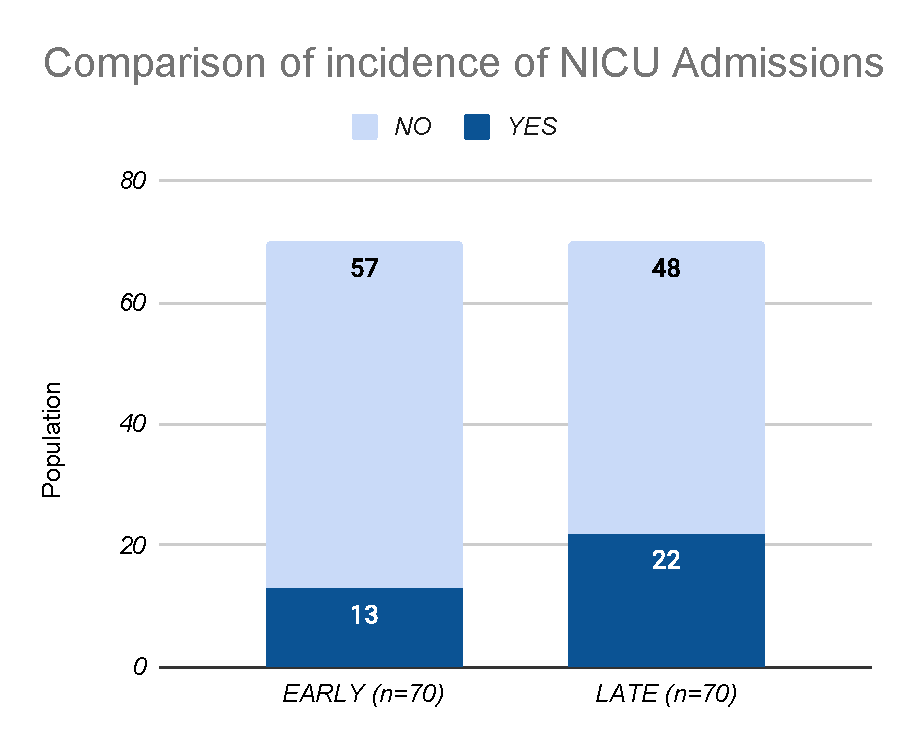
\includegraphics[width=0.95\textwidth]{figures/saranya_23}
\end{center}
\caption{Chart showing the incidence of NICU admission in the study population.}
\end{figure}
\clearpage

\begin{table}[ht]
\centering
\begin{tabular}{|l|c|c|c|}
\hline
\textbf{}                                                  & \multicolumn{1}{l|}{\textbf{MEAN(g)}} & \multicolumn{1}{l|}{\textbf{STD DEV(g)}} & \multicolumn{1}{l|}{\textbf{p-value}} \\ \hline
\begin{tabular}[c]{@{}l@{}}Early\\  Amniotomy\end{tabular} & 3017.34                               & 294.58                                   & \multirow{2}{*}{0.1597}               \\ \cline{1-3}
\begin{tabular}[c]{@{}l@{}}Late \\ Amniotomy\end{tabular}  & 2947.97                               & 285.91                                   &                                       \\ \hline
\end{tabular}
\caption{Table showing the the distribution of birth weight of the newborns in the study population.}
\end{table}

\begin{figure}[!hb]
\begin{center}
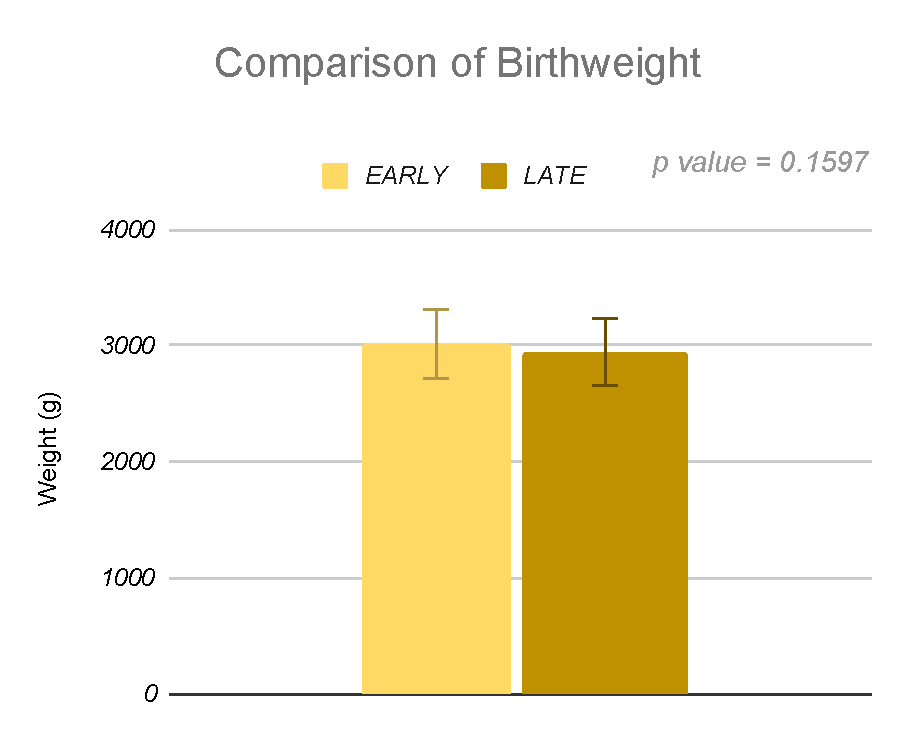
\includegraphics[width=0.95\textwidth]{figures/saranya_24}
\end{center}
\caption{Chart showing the the distribution of birth weight of the newborns in the study population.}
\end{figure}
\clearpage

\begin{table}[!ht]
\centering
\begin{tabular}{|l|c|c|c|c|}
\hline
\multicolumn{1}{|c|}{\textbf{APGAR}} & \textbf{EARLY (n=70)} & \textbf{(\%)} & \textbf{LATE (n=70)} & \textbf{(\%)} \\ \hline
$\leq$7                                   & 21                    & 30            & 24                   & 34.29         \\ \hline
\textgreater{}7                      & 49                    & 70            & 46                   & 65.71         \\ \hline
\end{tabular}
\caption{Table showing the APGAR scores  in the study population.}
\label{tab:my-table}
\end{table}

\begin{figure}[!hb]
\begin{center}
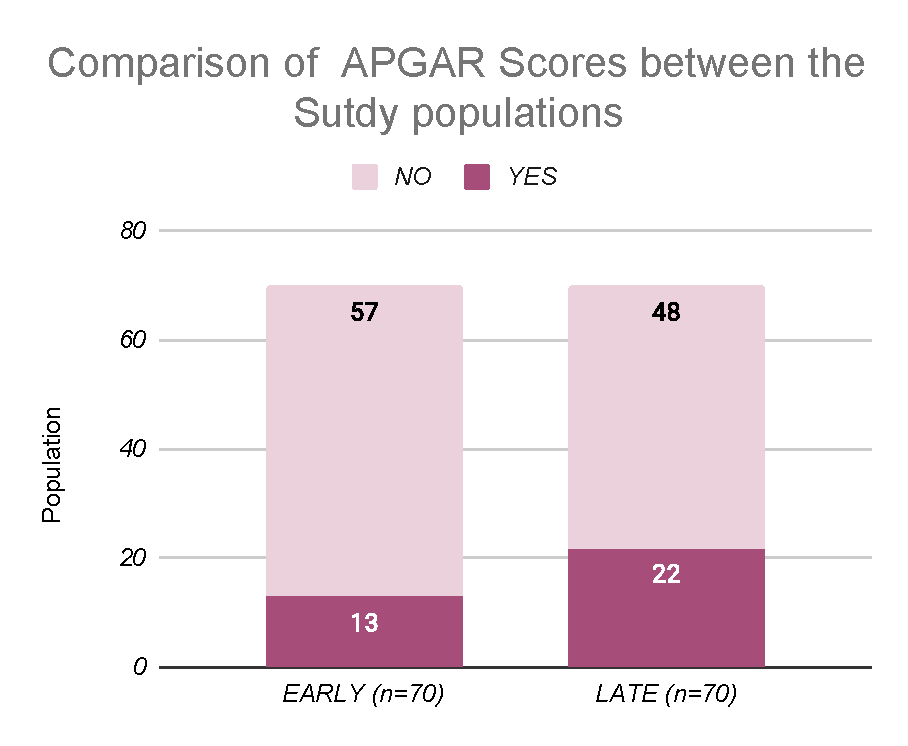
\includegraphics[width=0.95\textwidth]{figures/saranya_25}
\end{center}
\caption{Chart showing the APGAR scores  in the study population.}
\end{figure}

\clearpage

\begin{table}[ht]
\centering
\begin{tabular}{|l|c|c|}
\hline
\textbf{STILL BIRTH} & \textbf{EARLY(n=70)} & \textbf{LATE(n=70)} \\ \hline
YES                  & 0                    & 0                   \\ \hline
NO                   & 70                   & 70                  \\ \hline
\end{tabular}
\caption{Table showing the incidence of stillbirth in the study population.}
\end{table}

\begin{figure}[!hb]
\begin{center}
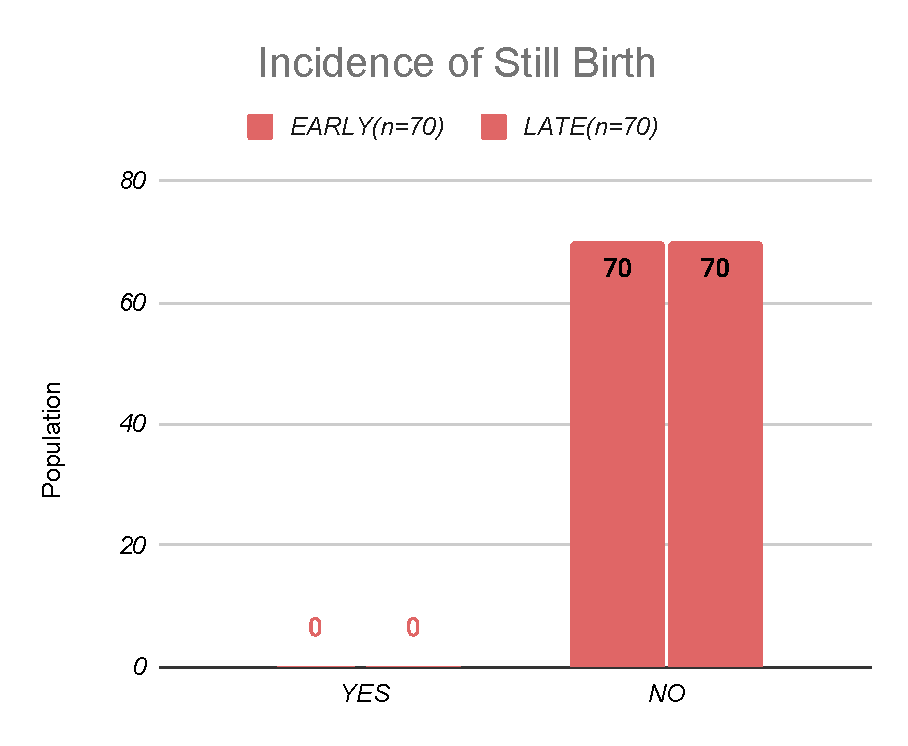
\includegraphics[width=0.95\textwidth]{figures/saranya_26}
\end{center}
\caption{Chart showing the incidence of stillbirth in the study population.}
\end{figure}
\clearpage

\null
\vfill
\begin{flushright}
    \section{DISCUSSION}
\end{flushright}
\hrulefill
\newpage

Out of 150 patients who were included in out study 36\% of the population were aged less than 21 years while the majority of around 57.33\% belonged to the ages between 21 and 30. A small but significant population of 6.67\% belonged to the age of 30 to 35years. 75\% of the study population were booked before the bleeding episode. 25\% of the study population were unbooked. These women were unbooked as pregnancy was diagnosed as a result of evaluation of the bleeding episode. 64\% of the women experienced bleeding for the first time in the current pregnancy while 35.33\% of the women had history of similar bleeding in the previous pregnancy. 

60.67\% of the study population were primigravida whereas 39.33\% were multigravidas. Among multigravidas 1.33\% were grand multigravidas. 14\% of the study population had bleeding episode before 6 weeks of gestation while 20\% had their first bleeding episode after 10 weeks. The majority of the population experience bleeding between 6 and 10 weeks. Most of the women experience mild spotting as described by them. These women constituted 48\% of the study population. 28\% of the women experience bleeding that they considered "more than spotting". 24\% of the women had bleeding that had clots.

In our study 84\% of the women with spotting in the first trimester continued their pregnancy beyond the viability period and hence were diagnosed as threatened abortion only. The number of women who continued their pregnancy dropped to 76.19\% in the more than spotting group while it was only 27.78\% in the women with clots. 6.94\% of the spotting group went on to have complete abortion while 11.9\% in the more than spotting group went on to have complete abortion. Interestingly none of the women in the clots group had complete abortion. 72.22\% of the clots group were diagnosed with incomplete abortion. This pattern may be because women with complete abortion expelled the fetus completely with minimal bleed afterwards and hence the number of women who reported the bleeding as clots was negligible. Only 1.39\% in the spotting group and 7.14\% in the more than spotting group had incomplete abortion.

5.56\% in the spotting group were diagnosed with ectopic pregnancy while there were none of the women in the more than spotting and clots group had ectopic pregnancy. A small number of women in the spotting and more than spotting group had molar pregnancies accounting for 1.39\% 5and 4.7\% respectively. None of the clots group were diagnosed with molar pregnancy.

Among the 61 pregnancies that progressed beyond the first trimester in the spotting only group 3.28\% ended up in miscarriage. The rest 96.72\% delivered a live neonate. 16.39\% delivered a preterm baby. 80.33\% delivered a term neonate.

32 women in the more than spotting group progressed beyond the first trimester. The number of miscarriages beyond first trimester doubled in the more than spotting group to 6.25\%. The majority of women who delivered a live neonate delivered prematurely accounting for about 78.13\% while term neonates constituted only 15.63\%. Only 10 women who had clots in the first trimester progressed beyond 12 weeks. 2 women of that 10 miscarried soon after the first trimester. 6 women delivered a preterm neonate while 2 delivered a term neonate.

Among the 41 women who delivered prematurely the NICU admission rate was 75.61\%. This rate was only 10.71\% in the term neonates. 12.2\% of the preterm neonates had a birthweight of less 1.5kg. 24.39\% of preterm neonates weighed between 1.5 and 2.5 and 63.41\% weighed between 2.6 and 3kg. None of the neonates who delivered prematurely weighed more than 3kgs. All the term neonates weighed above 1.5kg with more than 90\% of neonate weighing above 2.5kg. 62.5\% term neonates weighed between 2.5 and 3kg while 28.67\% weighed more than 3kg.

The number of preterm neonates who had an APGAR of $<$7 was little less than half of the total. 43.9\% preterm neonate had an APGAR of $<$7 and 56.10\% neonates had an APGAR of $>$7. As expected 90\% of term nenoates had an APGAR of $>$7 while the rest 10\% had an APGAR of $<$7. The low APGAR in these neonates may be due to the obstetrical complications seen in the mothers. 4.12\% of mothers had placental abruption, 15.46\% women had hypertensive disorders of pregnancy, 11.34\% had gestational diabetes mellitus, 8.25\% had both hypertension and diabetes and 9.28\% had placenta previa. Placental abruption was only seen in women who delivered at term possibly due to placental abnormalities that progressed as the pregnancy prolonged. All other complications were similar in both the term and preterm population.

48.45\% of the mothers delivered vaginally. 5.15\% had instrumental delivery and 46.39\% had caesarean delivery. Among the 97 neonates delivered 2(2.06\%) were still born and there were 5 neonatal deaths (5.15\%).

\newpage
\null
\vfill
\begin{flushright}
    \section{CONCLUSION}
\end{flushright}
\hrulefill
\newpage

CONCLUSION

\newpage
\null
\vfill
\begin{flushright}
    \section{BIBLIOGRAPHY}
\end{flushright}

\hrulefill
\newpage

\printbibliography[]

\newpage

\null
\vfill
\begin{flushright}
    \section{ANNEXURES}
\end{flushright}
\hrulefill
\newpage

\thispagestyle{empty}

%\begin{figure}[!h]
%    \centering
%    {\tiny \caption{Mifepristone Master sheet}}
%    \includegraphics[angle=90,scale=0.75]{images/mifepristone_master_sukitha.pdf}
%\end{figure}    

\clearpage

\thispagestyle{empty}

%\begin{figure}[!h]
%    \centering
%    {\tiny \caption{Mifepristone Master sheet}}
%    \includegraphics[angle=90,scale=0.75]{images/mifepristone_master_sukitha_2.pdf}
%\end{figure} 

\clearpage

\thispagestyle{empty}

%\begin{figure}[!h]
%    \centering
%    {\tiny \caption{Letrozole Master sheet}}
%    \includegraphics[angle=90,scale=0.75]{letrozole_master_sukitha_2}
%\end{figure} 

\clearpage

\thispagestyle{empty}

%\begin{figure}[!h]
%    \centering
%    {\tiny \caption{Letrozole Master sheet}}
%    \includegraphics[angle=90,scale=0.75]{images/letrozole2_master_sukitha_2.pdf}
%\end{figure} 

\clearpage

\begin{center}
    \textbf{CERTIFICATE OF APPROVAL}
\end{center}

%\begin{figure}[!h]
%    \centering
%    \includegraphics[scale=0.7]{ethical.jpeg}
%\end{figure}    
%
\clearpage

\textbf{PLAGIARISM CERTIFICATE}

\newpage

\textbf{PROFORMA}

Particulars

\begin{itemize}
    \item Name
    \item Age
    \item Address
    \item Phone no
    \item Religion
    \item Occupation
    \item Diet:Veg/Non Veg
    \item Education
    \item Date of admission
    \item Date of discharge
    \item Chief complaints
\end{itemize}

PAST History

\begin{itemize}
\item  Seizure disorder
\item  Hypertension
\item  Diabetes mellitus
\item  Stroke
\item  Ischaemic heart disease
\item  Pregnancy induced hypertension
\end{itemize}	

Family history

\begin{itemize}
\item Diabetes mellitus
\item Hypertension
\item Stroke
\item Ischaemic heart disease
\item Seizure disorder
\end{itemize}

Obstetric history

\begin{itemize}
\item  Gravida/parity
\item  Gestational age at the time of presentation
\item  Gestational age at the time of delivery
\end{itemize}

Treatment history

\begin{itemize}
\item  Antihypertensive medication
\item  Antiepileptic medication
\item  Anticoagulants
\end{itemize}

Others

General

\begin{itemize}
\item PR
\item B.P
\item RR
\item TEMP
\item WT
\item HT
\item BMI
\item Pallor
\item Icterus
\item Cyanosis
\item Edema
\item Lymphadenopathy
\item Clubbing
\end{itemize}

CNS examination

CVS examination

Respiratory system examination

GI examination

OUTCOME OF INDUCTION

\begin{itemize}
\item Complete abortion
\item Surgical interference
\end{itemize}

INDUCTION ABORTION INTERVAL

BLEEDING DURATION

DRUG SIDE EFFECTS

\begin{itemize}
\item Nausea
\item Vomiting
\item Diarrhoea
\item Dizziness
\item Headache
\item Abdominal pain
\item Fever
\item Chills
\end{itemize}

Investigations

\begin{itemize}
\item Hb
\item PBS
\item Hct
\item Coagulation profile
\item MCV
\item TLC
\item DLC
\item Platelet count
\item Blood urea
\item Sr.Creatinine
\item Urine protein
\item S.Uric acid
\item S.Bilirubin
\item SGOT
\item SGPT
\item Sr.ALP
\item Total Protein
\item Sr.LDH
\item Sr.Sodium
\item Sr. Potassium
\end{itemize}

Ultrasound to confirm gestational age

\newpage

\begin{center}
    \textbf{PATIENT CONSENT FORM}
\end{center}

\small
\textbf{Dissertation Topic:}
\study

Department: Dept. of Obstetrics and Gynaecology

Hospital Name: Govt. Raja Mirasudhar Hospital, Thanjavur Medical College 

\
Patient’s Name: \\
Patient’s Age \\
Patient's Ip No: \\


Mark the following (x) :
( )The nature of the study explained to me clearly. I have been given the opportunity to clear my queries regarding the procedure \\
( ) I am willingly participating in this study. At any point of time I can get out of this study without any further issues \\
( ) During the study period or after the completion of this study, the doctor can verify my medical records without my consent \\
( ) I am willing to participate in this study and I am accepting this in my full conscience \\

\vspace{30mm}
\begin{multicols}{2}
    \begin{flushleft}
        Patients Name\\
        Patients Signature
    \end{flushleft}

    \begin{flushleft}
        Investigator's Sign\\
        \name
    \end{flushleft}
\end{multicols}

\end{document}
